\documentclass[12pt]{report}
\usepackage[utf8]{inputenc}
\usepackage{graphicx}
\usepackage{float}
\usepackage{pgfgantt}
\usepackage{hyperref}
\usepackage{algorithm2e}
\usepackage[left=2cm,right=2cm,top=2cm,bottom=2cm]{geometry}

\usepackage[toc]{glossaries}
\usepackage{appendix}
\usepackage{cite}
\usepackage{mathptmx}
\makeglossaries


% Comments
\usepackage{color}
\usepackage[normalem]{ulem} %pour le format barré
\newcommand{\hcp}[1]{\textcolor{blue}{[#1]}}
\newcommand{\hcr}[2]{\textcolor{red}{\sout{[#1]} - \textcolor{blue}{ [#2]}}}
\newcommand{\hc}[1]{\textcolor{red}{[#1]}}
\newcommand{\hcc}[1]{\textcolor{green}{Pour info - [#1]}}

\begin{document}
	\begin{titlepage}
		
		\newcommand{\HRule}{\rule{\linewidth}{0.5mm}} % Defines a new command for the horizontal lines, change thickness here
		
		\center 
		\HRule \\[0.4cm]
		{ \huge \bfseries Report \\Representation and relative positioning from visual information}\\[0.4cm]
		\HRule \\[1.5cm]
		
		\begin{minipage}{0.4\textwidth}
			\begin{flushleft} \large
				\emph{Submitted by:}\\
				\textsc{Asma BRAZI}
			\end{flushleft}
		\end{minipage}
		~
		\begin{minipage}{0.4\textwidth}
			\begin{flushright} \large
				\emph{Supervised by:} \\
				\textsc{Cédric HERPSON}\\
			\end{flushright}
		\end{minipage}\\[4cm]
		
		
		{\large Laboratory of Computer Sciences, Paris 6 \\ Sorbonne University - Faculty of Sciences and Engineering}\\[3cm] 
		{\large June - July 2019 }\\[3cm] 
		
\includegraphics[width=0.6\textwidth]{res/logo.png}\\[1cm] 
		\vfill % Fill the rest of the page with whitespace
		
	\end{titlepage}
	

	\chapter{Abstract}
	
	\paragraph{}
	We carried out our internship at the Laboratory of Computer Sciences, Paris 6 (LIP6) under the supervision of Cédric Herpson, from June 3rd, 2019 until July 16th, 2019. The internship was mainly considered as a continuation of works that we carried out during a university project (PANDROIDE) in our first Master's degree. 
	
	\paragraph{}
	Our previous works presented a naive approach of object recognition and exploration strategy that allowed an autonomous robot with a camera to roughly build its environment. The environment is close and composed of walls where the robot was able to locate itself. In addition, we could ask the robot to search for a specific object, and the robot was able to accomplish that task. Nevertheless, the conducted works assumed some hypotheses which did not make the exploration strategy generic.
		
	\paragraph{}
	During this internship, we focused the most on improving the exploration strategy, to no longer depend on certain hypotheses. For example, in our previous works, we had some specific objects placed on corners to indicate to the robot that there is a corner at this spot. This hypothesis allowed the robot not to perform image processing to detect corners. 
	
	\paragraph{}
	Our new strategy does not depend anymore of these objects. But, it exploits some visual information like contours. Also, the information provided by the robot's sensors is taken into account. We developed so a strategy where no knowledge of the environment is necessary, and no hypothesis helping the robot building its environment are considered.
	
	\chapter{Acknowledgments}
	\paragraph{}
	I would like to deeply thank my supervisor, Cédric Herpson, for his guidance and help, his presence and his trust in me to lead the initiative in my work. 
	
	I can say that I have been truly lucky to have Cédrid Herpson as a supervisor who cared so much about my work, although he had a lot of work ahead of him. 
	
	
	\tableofcontents
	\chapter{Introduction}
	\paragraph{}
	When an autonomous robot navigates in a structured or unstructured environment, it should be able to build a map representing this environment, to localize itself in it and to define a safe path to move from a place to another one.
	
	\paragraph{}
	There are a varied applications of the robot navigation. Such as surveillance, cleaning, transportation tasks...etc. As a result, the number of contributions of researchers in this field keeps going up \cite{bonin-font_visual_2008}.
	
	\paragraph{}
	Our project aims to enable the Thymio robot\footnote{An educational programmable robot} with a camera to build roughly  its environment. The environment is close and it is composed of walls where the robot is able to locate itself. 
	
	Unlike our previous work where we had some landmarks helping the robot in the localization of corners, we develop a strategy totally generic. With this strategy, the robot can manage to build its entire environment autonomously.
	
	
	\section{Outline of this report}
	\paragraph{}
	The remaining chapters are organized as follows:
	\begin{itemize}
		\item Chapter 4: Summarize of the state of art.
		\item Chapter 5: Explanation of the solution.
		\item Chapter 6: Discussion of the solution.
		\item Chapter 7: Conclusion of our works and suggestion of future works.
	\end{itemize}: 
	
	
    \chapter{Reviews of Existing Work}
	
	\paragraph{}
	The main purpose of our works is to improve the functionalities developed previously. These functionalities allowed the autonomous robot to move in its environment and explore it. The visual information brought by the exploration is used to build a virtual 3D representation of this environment, and to recognize a target object. The target object is an object from the knowledge database. It is specified by the user, at the launching of the application.
	
	\paragraph{}
	In short, our previous strategy can be summarized as follows:
	\begin{itemize}
		\item At each move, the autonomous robot took a picture and analyzed it.
		\item The analysis of the picture brought new knowledge to the autonomous robot.
		\item With this new knowledge, The autonomous robot was able to represent its environment and to recognize the target object.
	\end{itemize}

	\paragraph{}
	However, we assumed some hypothesis that facilitated the process of the exploration. For example, we placed some objects in each corner of the environment and every time the autonomous robot met these objects, it concluded that this was a wall end. So the autonomous robot relied on these objects to decide whether or not it finished exploring the current wall. 
	
	\paragraph{}
	To no longer depend on this hypothesis, we present in our works another manner to construct the environment. Firstly, the autonomous robot does not try to detect the walls anymore by detecting corners. Instead, it takes a picture, analyzes it to extract the contours of the environment. With these contours, the robot decides if it is in front of a face, or if it still has a way to go...etc.
	
	By this way, the autonomous robot gathers the analysis's results to estimate the dimensions of the walls.
	
	\paragraph{}
	Regarding the lengths and heights of walls, we globally estimate them in the same way as in the previous works. Nevertheless, the algorithm behind the calculations that we will develop later, is a little bit different. 

    \chapter{Realization}
    \paragraph{}
    We suppose that the robot is situated in a closed environment, and it has been informed about the target object to search. 
	\section{Exploration strategy}
	 \subsection{Image processing}
	 \paragraph{}
	 The first task of the autonomous robot is to represent roughly the environment, using visual information. For walls detection, we distinguish three types of segments on the picture taken by the autonomous robot:
	 \begin{itemize}
	 	\item Vertical segment which makes almost 90 degrees with the X-axis.
	 	\item Horizontal segment which makes almost 0 degree with the  X-axis.
	 	\item The rest of segments with the other angles.
	 \end{itemize} 
	 
	 
	 \paragraph{}
	 In the sections to come, we present the different strategies that we have developed and the one we have particularly kept.
	 
	 \subsubsection{Corners-based detection}
	 \paragraph{}
	 We have begun with a strategy based on corners detection. Where we kept the same exploration strategy as in our previous works. But, we replaced only the part of corners detection. So instead of detecting a specific objects substituting the corners, we tried two methods. We developed an approach based on \textit{segments intersection} and we used a pre-defined  method from OpenCV for \textit{corners detection}. These two methods were used under a certain constraints, to decide whether it is a corner or not.
	 \paragraph{}
	 Defining these constraints is not that easy. For example, it is getting arduous if we have a textured floor or walls. So the method consider all the intersection points of the walls and the floor as corners. 
	
	 Also, if the floor and the walls have almost the same color, the segment separating the wall from the floor may not be detected.
	 
	 As a result, these methods detect a lot of features which are not all correct corners.
	 
	 \paragraph{}
	 On the other hand, if we assume that corners are situated in most cases on the bottom of the image, this assumption becomes incorrect if the robot is so far from the corner. In this case, the corner is situated on the top of the image. The figure below explicits that:
	 	\begin{figure}[H]
	 	\begin{center}
	 		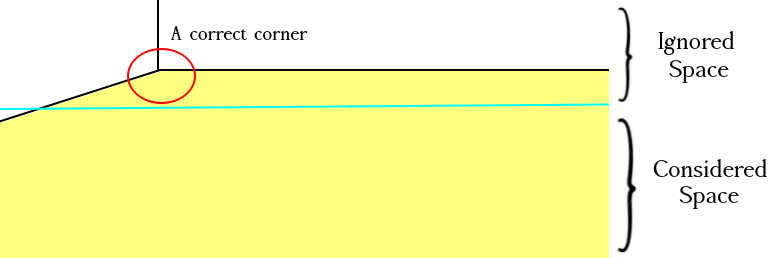
\includegraphics[scale=0.6]{res/start1_c1.png}
	 		\caption{An ignored corner because of the corners placement constraint}
	 	\end{center}
	 \end{figure}
	 \paragraph{}
	 As a result, this corner will be ignored as it is not situated on the bottom of the image.
	 
	 \paragraph{}
	 These particular pictures taken by the autonomous robot make the strategy not really captivating, because it is sensitive to the autonomous robot's position.
	 
	 \subsubsection{Non corners-based detection}
	 \paragraph{}
	 After encountering some difficulties to detect the right corners, we decided to ditch this strategy because it was impractical. 
	 
	 \paragraph{}
	 The next idea is to consider the segments on the 3 axis X,Y and Z. The vertical (resp. horizontal) segments are used to estimate the walls height (resp. width). However the diagonal segments detected indicate that there is a depth. Knowing that a certain depth exists on the image, guarantees to the autonomous robot that there is still space between them and the wall in front. So, it can always move forward.
	  
	  \paragraph{}
	  We have used the algorithm: \textit{Line Segment Detector} (LSD) to detect straight contours on the image \cite{grompone_von_gioi_lsd:_2012}. At each pixel of the image, LSD estimates the angle of the gradient. After that, the pixels sharing nearly the same angle of gradient are merged into regions. The connected regions are called \textit{line support regions}. Then, the algorithm keeps some of these \textit{line support regions} to be a \textit{line segment}.
	  
	  the picture below shows an image on which the LSD was applied and as a result, the \textit{line support regions} that were detected.
	  	\begin{figure}[H]
	  	\begin{center}
	  		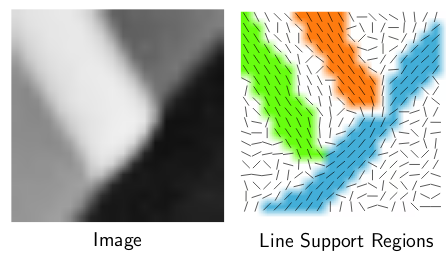
\includegraphics[scale=0.6]{res/lsr.png}
	  		\caption{Line Support Regions. Adapted from "Rafael Grompone von Gioi, Jérémie Jakubowicz, Jean-Michel Morel, and Gregory Randall, LSD: a Line Segment Detector, Image Processing On Line, 2 (2012)" }
	  	\end{center}
	  \end{figure}
  \paragraph{}
  So, on each picture taken by the autonomous robot, we apply LSD to obtain segments. After that, the segments are classified into groups: the verticals, the horizontals and the diagonals, up to a certain tolerance $\epsilon$. Each group of segments is used for a certain purpose for the navigation. Then, in each group, we merge the closet segments up to a certain tolerance $\lambda$, in order to get longer segments, and we keep only the longest one from each group. 

The horizontal segments which are situated on the top of the image are ignored. We assume that theses segments represent a ceiling. We do not risk anything by ignoring theses segments because, even if the segments represent a frontier between the floor and far wall. We built a strategy where the autonomous robot gets closer to the far wall to construct it.
    \subsection{3D map building}
    
    \paragraph{}
    We remind that our goal is to build a rough 3D representation of the environment and look for the target object. We represent the environment by defining the walls composing it. The detection of walls is based on LSD's segments.
    
    \paragraph{}
    Depending on the autonomous robot's position, the picture obtained may in one of the general cases showed in the picture below. 
    
    
    	\begin{figure}[H]
    	\begin{center}
    		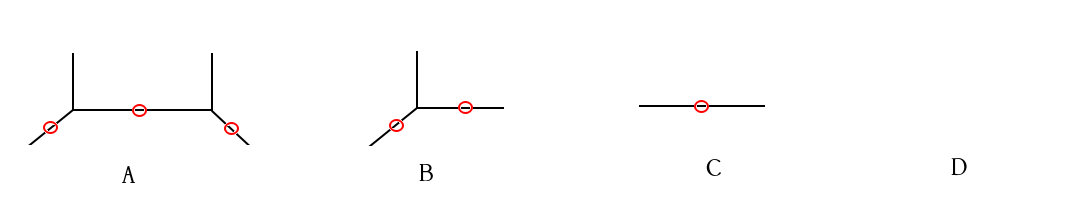
\includegraphics[scale=0.6]{res/cases_seg.png}
    	\end{center}
    \end{figure}
 \paragraph{}
 The useful information that we can retrieve from each case is as follows:
 \begin{itemize}
 	\item Case A: 3 types of segments are detected, an horizontal one and 2 diagonals on 2 opposing walls.
 	\item Case B and C: 2 types of segments (horizontal and diagonal) sharing an endpoint are detected.
 	\item Case D: An horizontal segment is detected.
 	\item Case E: Any segment is detected.
 	
 \end{itemize}
 \paragraph{}
 We mention that the vertical segments are used only to set the height of walls, they are not used in the exploration strategy because the autonomous robot is moving only along the X and Z axis.
 \subsection{Navigation}
     \paragraph{}
 Navigation is the determination of an adequate and secure path for the autonomous robot, to move from a starting spot to a target one \cite{bonin-font_visual_2008}.
 \paragraph{}
 On the basis of visual information, the autonomous robot is able to define its next decision. The decision may be to:
 \begin{itemize}
 	\item Stop if the target has been found or if the robot has explored the entire environment, without spotting the target.
 	\item Avoid obstacles.
 	\item Move back, move forward and rotate to continue exploring.
 \end{itemize}

\subsubsection{Obstacle avoidance}
\paragraph{}
In our previous work, when the autonomous robot decided to move forward, it did not check progressively while moving whether there is an obstacle or not. But, it verified if there is an obstacle when it stopped moving. The drawback of such a decision is that the autonomous robot is not able to distinguish between its last position and the one after moving.
\subsubsection{Strategy}
\paragraph{}
As there are a lot of cases of movements according to the visual information, we try to summarize theses cases using an activity diagram shown in the figure below. In this diagram, the green boxes represent a physical movement of the autonomous robot, and the blue cases represent treatments. 

\paragraph{}
We assume that the user has already mentioned the name of the object to find, and that the robot is situated in a close environment.

If we start with the initial point of the diagram, we can see that the autonomous robot begins by taking a picture and analyzes it. After that, it extracts the visual information from the taken picture and sends them to the computer, where the orders of movements are given. 

From the collected information, if the target has been found, the autonomous robot stops. Otherwise, If there are any segments detected, each of these segments is represented by a wall and added to the 3D map.
\paragraph{}
At the end of the treatment, a movement is ordered to the autonomous robot (rotate, move back...etc). Then, it regains from the beginning until it stops.
\newpage
	\begin{figure}[H]
	\begin{center}
		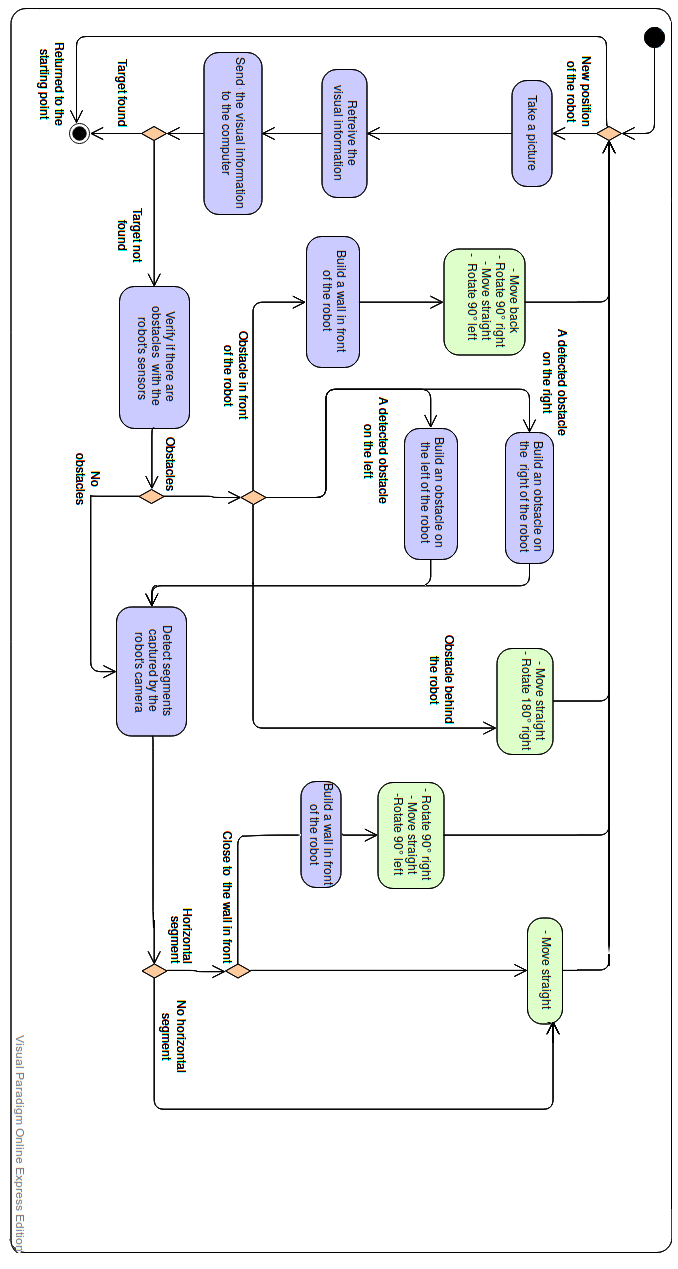
\includegraphics[scale=0.55]{res/order_processing.png}
		\caption{Activity diagram of the exploration strategy}
	\end{center}
\end{figure}
\newpage
	

	\chapter{Testing}
	\paragraph{}
	We have realized different tests by varying the environment, beginning by a simple rectangular environment to a complex environment containing corridors, and where there a some obstacles. 
	
	\section{Image processing}
	
	\section{3D map building}
	
	\chapter{Conclusion, Limitation and Future work}
	\section{3D Object recognition}
	\chapter{References}


	\appendix
	\chapter{List of components}
	\section{Thymio II}
	\textbf{Description} 
	\paragraph{}
	Thymio II is a mobile robot dedicated to the education field. It has many sensors for different purposes. These sensors covered:infrared receiver,proximity, 3 axis accelerometer, ground sensors for line following...etc.
	\\ \\
	\textbf{Data sheet} 
	\paragraph{}
	\url{https://www.generationrobots.com/fr/401213-robot-mobile-thymio-2.htmlURL}
	\begin{figure}[H]
		\begin{center}
			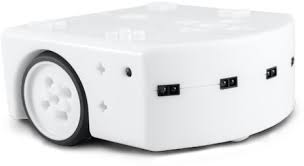
\includegraphics[scale=0.6]{res/thymio.jpg}
		\end{center}
	\end{figure}
	\section{Raspberry-Pi}
	\textbf{Description}
	\paragraph{}
	The Raspberry-Pi is a s single-board computer with wireless LAN and Bluetooth connectivity. It needs a micro USB power supply (2.1 A) in order to be plugged into a power-bank. It has 1GB RAM, 4 USB 2 ports, Full size HDMI, 100 base Ethernet and including a quad core 1.2GHz Broadcom BCM2837 64bit CPU.\\ \\
	\textbf{Data sheet} 
	\paragraph{}
	\url{https://www.raspberrypi.org/products/raspberry-pi-3-model-b/}
	\begin{figure}[H]
		\begin{center}
			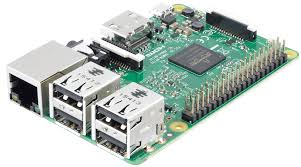
\includegraphics[scale=0.6]{res/raspberry.jpg}
		\end{center}
	\end{figure}
	\section{Raspberry-Pi Camera}
	\textbf{Description}
	\paragraph{}
	The Raspberry-Pi Camera delivers a 5MP resolution image, and 1080p HD video recording at 30 frame/second. It plugs into the Camera Serial Interface connector on the Raspberry-Pi. \\ \\
	\textbf{Data sheet} 
	\paragraph{}
	\url{https://uk.pi-supply.com/products/raspberry-pi-camera-board-v1-3-5mp-1080p?lang=fr}
	\begin{figure}[H]
		\begin{center}
			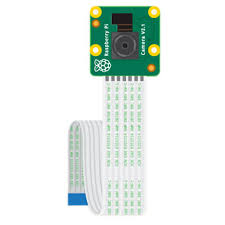
\includegraphics[scale=0.6]{res/camera.jpg}
		\end{center}
	\end{figure}
	\section{Power-bank}
	\textbf{Description}
	\paragraph{}
	For testing, we used RAVPower powerbank to power the Raspberry-Pi. It has 2A input which can charge the 6700 mAh portable charger. this feature guarantees that the Raspberry-Pi's services work correctly. \\ \\
	\textbf{Data sheet} 
	\paragraph{}
	\url{https://www.ravpower.com/p/Ravpower-6700mAh-Portable-Charger.html}
	\begin{figure}[H]
		\begin{center}
			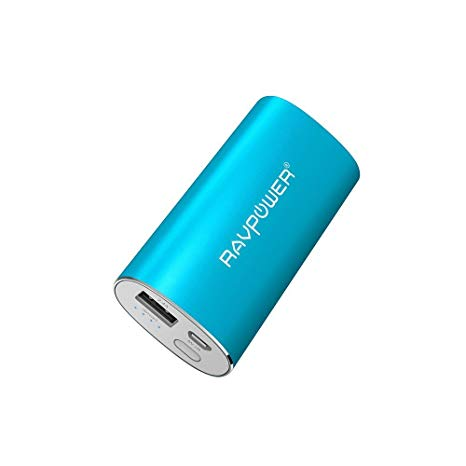
\includegraphics[scale=0.6]{res/power.jpg}
		\end{center}
	\end{figure}
	\chapter{Beginning of eventual future work}
	\section{3D Object recognition}
	\paragraph{}
	This project may improved for 3D Object Recognition. Currently, the objects to detect are only in 2D. Obviously, it will be more interesting to make the autonomous robot able to detect 3D object, and to integrate them to the 3D virtual map.  
	
	\paragraph{}
	In this case, we have begun to work on 3D object recognition, and we have thought about a solution where Deep Learning is used. For that, 
\end{document}